\documentclass[a4paper, 12pt]{article}

\usepackage[T1]{fontenc}
\usepackage[utf8]{inputenc}
\usepackage{lmodern}
\usepackage[english]{babel}
\usepackage{braket}
\usepackage{csquotes} 
\usepackage{graphicx}
\usepackage{gensymb}
\usepackage{siunitx}
\usepackage{wrapfig}
\usepackage{geometry}
\usepackage{textcomp}
\usepackage{float}
\usepackage{caption}
\usepackage{subcaption}
\usepackage{booktabs}
\usepackage{longtable}
\usepackage{amsmath}
\usepackage{xcolor}
\usepackage{physics}
\usepackage{tikz}
\usepackage{bookmark}
\usepackage{mathtools}
\usepackage{hyperref}
\usepackage{quantikz}

\hypersetup{
    colorlinks=true,
    citecolor=blue,
    filecolor=black,
    linkcolor=blue,
    urlcolor=black,
    pdfauthor={Rishik R},
    pdftitle={Rubidium Saturation Absorption Spectroscopy},
    pdfkeywords={Quantum Entanglement, Physics, RRI, SSSIHL}
}

\setlength{\parskip}{0.5em} 
\setlength{\parindent}{1.5em}  

\usepackage{setspace}
\renewcommand{\baselinestretch}{1.3}

\geometry{top=1.7cm, bottom=1.7cm, left=1.7cm, right=1.7cm}

\begin{document}

\begin{titlepage}
    \centering
    \vspace*{1.5cm}

    {\LARGE \textbf{Saturation Absorption Spectroscopy}}\\
    {\LARGE \textbf{of Rubidium}}\\[1.5cm]

    {\Large Rishik R}\\[0.2cm]
    {\large (M.Sc. Physics, SSSIHL, PSN Campus)}\\[0.2cm]
    {\large (as a Visiting Student at RRI)}\\[2cm]

    \begin{minipage}{0.5\textwidth}
        \centering
        
\includegraphics[width=\textwidth]{sssihl.jpeg}
    \end{minipage}
    \hfill
    \begin{minipage}{0.45\textwidth}
        \centering
        
\includegraphics[width=\textwidth]{rri.jpg}
    \end{minipage}\\[1.5cm]

    {\Large Under Prof. Saptarishi Chaudhuri,}\\[0.1cm]
    {\large Quantum Mixtures (QuMix) Lab}\\[1.5cm]
    {\large May -- June, 2025}\\[0.5cm]

    \vfill
\end{titlepage}

\newpage
\tableofcontents
\newpage

\section*{Acknowledgements}
Prior to this visiting student program, I held two convictions:

\begin{enumerate}
    \item Quantum technologies would be the direction I'd go in the future because it has \textit{a lot} of physics.
    \item Optics is the direction I definitely wouldn't go in the future because it has \textit{too little} physics.
\end{enumerate}

However, this visiting student program has made me question my bias, and I have come to appreciate optics wholeheartedly. This lab has shown me not only several experimental details that often go unnoticed, but also taught me to value the physical aspects of every setup—for everything physical conveys physics that is beautifully appreciable.

Since everything in this lab runs on optics, I gracefully accepted that I must confront my unscientific bias toward this field of lenses and mirrors—until I eventually loved what I was doing.

This program has graciously introduced me to countless concepts and ideas that I am slowly beginning to appreciate. It has also gifted me a new passion: Quantum Optics.

I would like to acknowledge the tremendous efforts of my labmates during this program. Anirban (da) for introducing me to ultra-cold atoms and BECs, Nilanjan (da) for introducing me to OAM modes of light and DMDs, Sayari (di), Abhishrutha (di), and Bhagyashri (di) for guiding me through atomic physics—particularly hyperfine structure—along with many helpful suggestions and discussions that brought clarity to experimental approaches.

Sai Vighnesh and Sai Varshini, for the innumerable conversations that made me question my choices—both in physics and in metaphysics. Prof. Saptarishi Chaudhuri, for nudging me in the right direction, for helping me understand the importance of experimental technique, and for offering me this wonderful opportunity—along with Dr. Muthu and Dr. K. Vijay Sai.

Finally, I would like to appreciate the magnanimous efforts of the Raman Research Institute in introducing students from across the country to new cultures, new relationships, and new frontiers of science.

Raman's legacy still lives on beautifully through the work carried out at RRI.


\newpage

\section{Introduction}
In a given atomic system, atoms move with different velocities. This leads to Doppler broadening. SAS is an experimental technique that eliminates this Gaussian broadening, giving rise to the thinnest possible linewidth. Typically in SAS:
\begin{itemize}
  \item A strong pump beam saturates the transition for atoms with zero velocity component along the laser axis.
  \item A weaker probe beam measures the absorption.
\end{itemize}

When the pump and probe are at the same frequency and the atom is stationary along the beam axis ($v=0$), both beams are resonant with the same group of atoms, leading to a sharp dip (called the \textit{Lamb dip}) in the spectrum.

\section{Saturation Absorption Spectroscopy (SAS)}
SAS, as mentioned above, is an elegant experimental technique that eliminates Doppler broadening caused by atomic motion, yielding the thinnest possible linewidth. A notable advantage of SAS is that it works even at room temperature and above, eliminating the need to cool the atoms.

To truly appreciate SAS, we take a pedagogical path—starting from the fundamentals and gradually understanding them in the context of SAS.

\subsection{Doppler Effect}
The Doppler effect is the change in frequency of a wave due to the relative motion between the source and the observer. We illustrate this using our scenario of lasers and atoms. To simplify, we consider two frames of reference: the \textbf{lab frame} and the \textbf{rest frame}.

The lab frame is the one in which the observer sees the atoms moving. In this frame, the laser frequency is $h\nu_0$. The rest frame is a frame moving with the atoms—essentially a coordinate system fixed at the atom’s center of mass.

Now, consider a laser beam propagating to the right (generally called the \textit{probe}). Atoms moving in the same direction as the laser beam experience a lower frequency—i.e., the beam is red-shifted in their frame, with frequency $h\nu_{\text{red}}$. Conversely, atoms moving opposite to the direction of the beam experience a higher frequency—i.e., a blue shift, with frequency $h\nu_{\text{blue}}$.

Atoms whose velocity component along the direction of the laser beam is zero observe the laser at its lab-frame frequency $h\nu_0$ (these atoms can also be moving perpendicular to the beam). 

\begin{figure}[htbp]
    \centering
    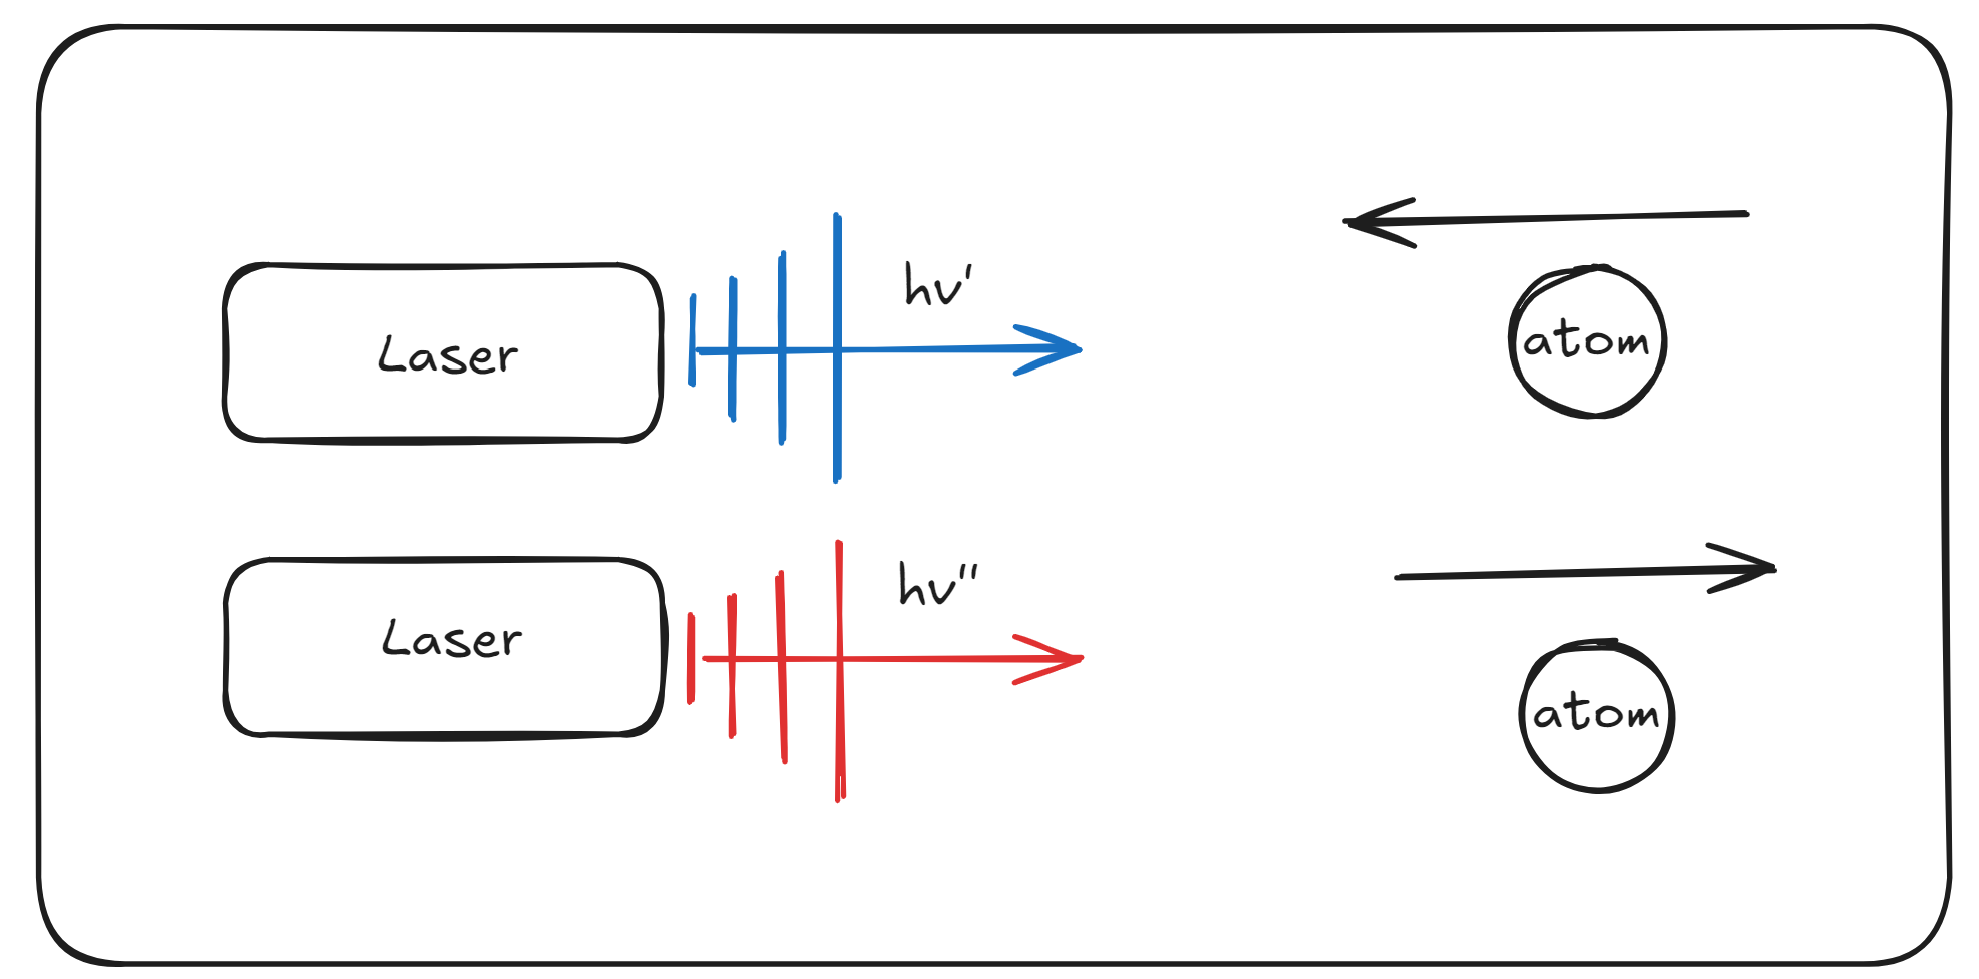
\includegraphics[width=0.7\textwidth]{doppler-shift.png}
    \caption{Simplified illustration of Doppler shift as seen by the atom depending on its relative motion to the source.}
\end{figure}

The above can also be understood from the mathematical relation:
\[
    \omega' = \omega - kv
\]
where 
$\omega'$ is the Doppler-shifted frequency, $\omega$ is the original lab-frame laser frequency, $k$ is the wave vector, i.e., $k = 2\pi/\lambda$, and $v$ is the velocity of the atoms.

So, the takeaway is that atoms do not necessarily absorb incoming radiation at the laser’s original frequency. Only if the Doppler-shifted frequency matches the resonant frequency will they absorb the incoming radiation. 

\subsection{3D Maxwell-Boltzmann Distribution}
In 3D, the total speed is related to the x, y, and z components (which are independent) as:
\[
    v^2 = v_x^2 + v_y^2 + v_z^2
\]
From this, we obtain the 3D Maxwell-Boltzmann distribution of velocity:
\[
\boxed{
f(\mathbf{v}) = \left(\frac{m}{2 \pi k_B T}\right)^{3/2} \exp\left( - \frac{m (v_x^2 + v_y^2 + v_z^2)}{2 k_B T} \right)
}
\]
And the corresponding speed distribution:
\[
\boxed{
f(v) = 4 \pi \left(\frac{m}{2 \pi k_B T}\right)^{3/2} v^2 \exp\left( - \frac{m v^2}{2 k_B T} \right), \quad v \geq 0.
}
\]

The main differences between these distributions are:
\begin{itemize}
    \item The speed distribution peaks at a non-zero value (the \textit{most probable speed}), which depends on temperature:
    \[
        v \simeq \sqrt{\frac{k_B T}{m}}.
    \]
    
    \item The velocity distribution is symmetric in each component because atoms do not have a preferred direction. As a result, the probability of an atom moving in a given direction is the same as that of moving in the opposite direction. Hence, the distribution is symmetric. The speed distribution, however, includes a multiplicative factor of $v^2$ and is not symmetric.
\end{itemize}

\begin{figure}[htbp]
    \centering
    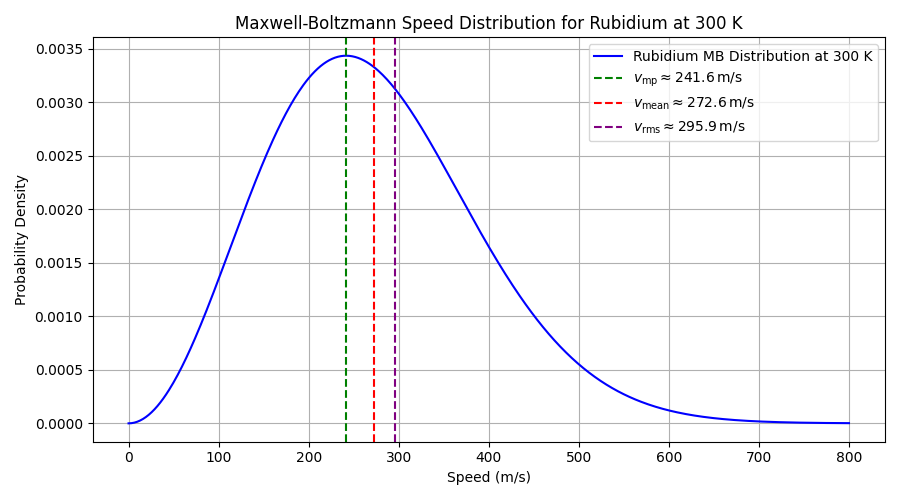
\includegraphics[width=0.9\textwidth]{mb-speed.png}
    \caption{Maxwell-Boltzmann speed distribution}
\end{figure}

\begin{figure}[htbp]
    \centering
    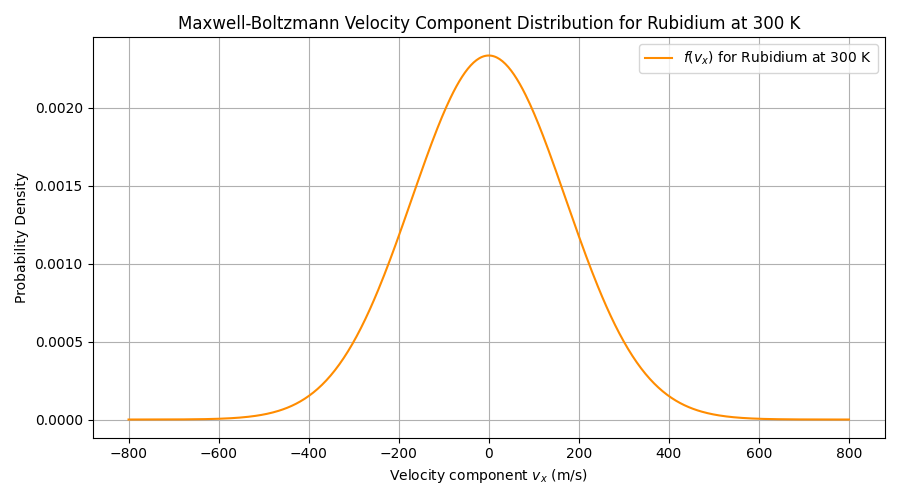
\includegraphics[width=0.9\textwidth]{mb-velocity.png}
    \caption{Maxwell-Boltzmann velocity distribution ($V_x$)}
\end{figure}

\newpage

\subsection{The SAS Spectrum}
One of the primary factors affecting the SAS spectrum is the intensity of the laser beams. The transition rate for a given intensity is denoted by:
\[
    \gamma = \alpha I
\]
where $I$ is the intensity of the laser beam. The coefficient $\alpha$ follows the relation:
\[
    \alpha = \alpha_0 \mathcal{L}(\nu, \nu_0)
\]
where $\mathcal{L}(\nu, \nu_0)$ gives the Lorentzian frequency dependence:
\[
    \mathcal{L}(\nu, \nu_0) = \frac{1}{1 + 4(\nu - \nu_0)^2/\Gamma^2}.
\]
The maximum transition rate occurs when $\nu = \nu_0$, and the corresponding intensity is called the saturation intensity $I_{\text{sat}}$:
\[
    I_{\text{sat}} = \frac{\gamma}{\alpha_0} \simeq 1.6\,\mathrm{mW/cm^2}
\]
with $\alpha_0 \simeq 2 \times 10^{6}\,\mathrm{m^2/J}$ for Rubidium transitions. At this intensity, atoms are equally likely to decay by spontaneous emission or by stimulated emission.

In our experiment, we varied the intensity and observed its effects on the full width at half maximum (FWHM) of the transition peaks.

\subsubsection{Experimental Setup}
\begin{figure}[htbp]
    \centering
    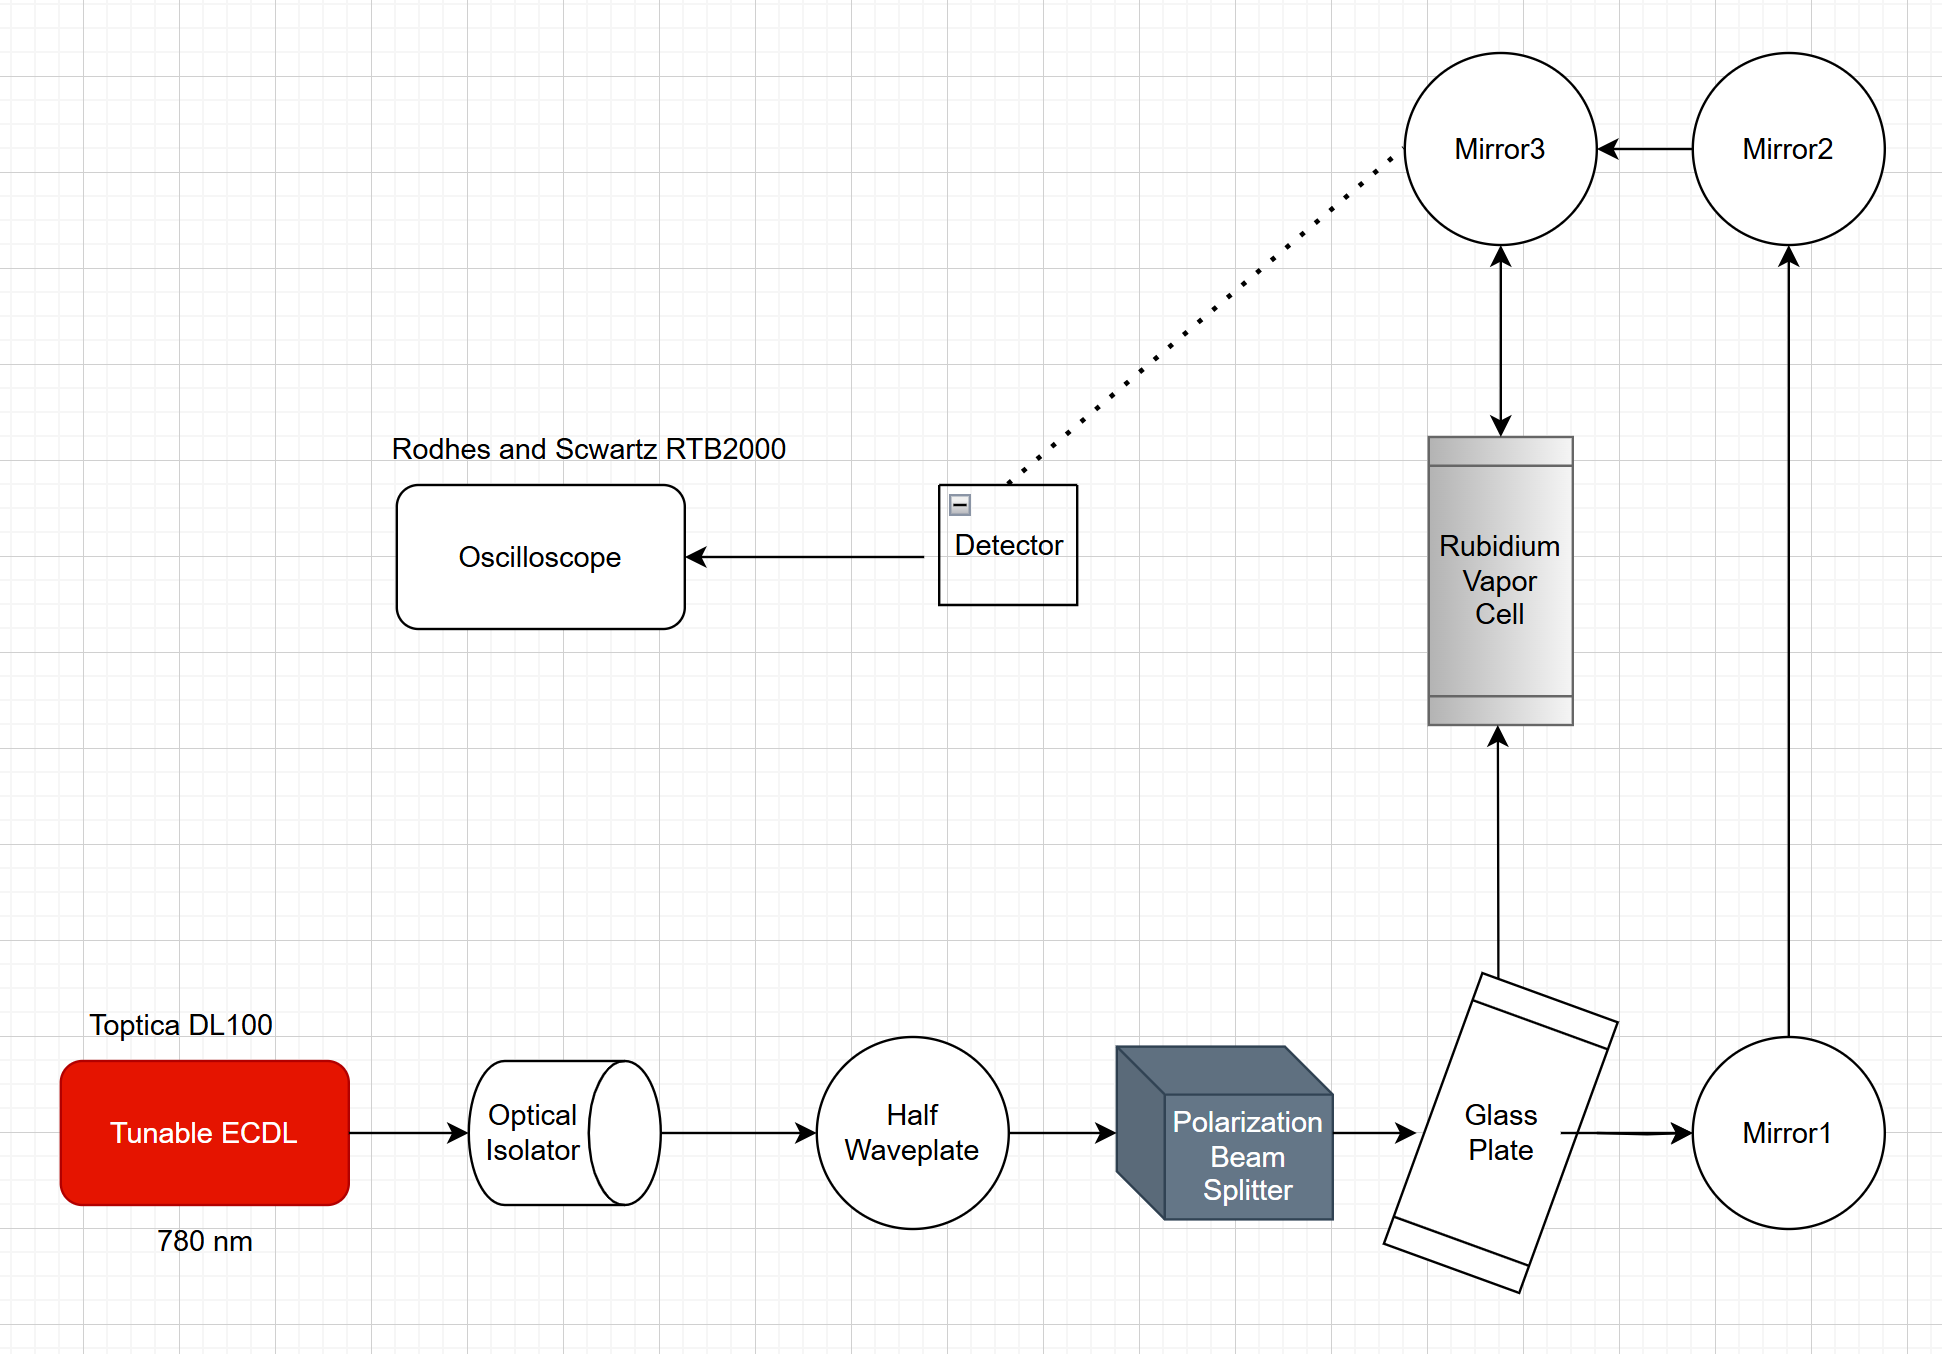
\includegraphics[width=0.7\textwidth]{experimental-setup.png}
    \caption{Saturation Absorption Spectroscopy experimental setup.}
    \label{fig:label}
\end{figure}


The setup is relatively simple but yields powerful results. A laser beam passes through a half-wave plate and a polarizing beam splitter (PBS), splitting the beam into two: one proceeds directly to the Rb vapor cell (probe), while the other reflects via mirrors M1, M2, and M3 to pass back through the cell (pump). The probe beam is weaker than the pump, although both originate from the same laser and thus have identical frequencies.

The laser frequency is scanned using two knobs:
\begin{itemize}
    \item \textbf{Scan Amplitude} — controls the frequency range, by changing the distance of the cavity.
    \item \textbf{Scan Offset} — controls the central frequency.
\end{itemize}

With the beams properly aligned (counter-propagating), the frequency scan interacts with atoms in the vapor cell. 

For example, consider atoms moving to the left that resonate with the pump beam. They absorb pump photons but are not in resonance with the probe, so they don’t absorb it. However, because the velocity distribution is symmetric, there exist atoms moving with the same speed to the right. These atoms will resonate with the probe beam instead and absorb it.

This happens across all velocity classes, except those with zero velocity along the beam axis. These atoms, which are most abundant (as shown in the Maxwell-Boltzmann distribution), see both beams in resonance. They absorb primarily from the intense pump beam, and the probe beam, finding the atoms already excited, passes through without interaction.

This results in a sudden increase in transmission—a sharp dip (Lamb dip) in the absorption signal, corresponding to zero-velocity atoms being saturated. The detector measures this increased transmission, allowing us to estimate both the resonant frequencies and the population of these atoms.

\section{Rubidium Atoms}
In a typical Rubidium vapor cell, two isotopes are present: $^{85}$Rb (72.2\%) and $^{87}$Rb (27.8\%). $^{87}$Rb has a half-life of $4.97 \times 10^{10}$ years, while $^{85}$Rb is effectively stable. The Gaussian peaks in the SAS spectrum reflect this isotopic distribution. In the D2 transitions, the smaller valley on the left corresponds to $^{87}$Rb, and the larger valley on the right corresponds to $^{85}$Rb, consistent with their natural abundances.

\subsection{Hyperfine Structure}
Fine structure results from the coupling between the electron’s orbital angular momentum ($\vec{L}$) and its spin angular momentum ($\vec{S}$), forming the total angular momentum $\vec{J}$:
\[
    |L - S| \leq J \leq |L + S|.
\]

In the ground state of $^{87}$Rb, $L = 0$, $S = 1/2$, so $J = 1/2$. In the first excited state, $L = 1$, $S = 1/2$, so $J = 1/2$ and $3/2$.

Thus, the $5^2S_{1/2} \rightarrow 5^2P_{1/2}$ transition is the D$_1$ line, and the $5^2S_{1/2} \rightarrow 5^2P_{3/2}$ transition is the D$_2$ line.

Hyperfine structure arises from the coupling between the total electronic angular momentum $\vec{J}$ and the nuclear angular momentum $\vec{I}$:
\[
    \vec{F} = \vec{J} + \vec{I}
\]
\[
    |J - I| \leq F \leq |J + I|.
\]

In the ground state of $^{87}$Rb: $J = 1/2$, $I = 3/2$ $\Rightarrow$ $F = 1, 2$.

In the D$_2$ excited state ($5^2P_{3/2}$), $F = 0, 1, 2, 3$. For the D$_1$ excited state ($5^2P_{1/2}$), $F = 1, 2$.

A similar analysis applies to $^{85}$Rb.

\begin{figure}[h!]
    \centering
    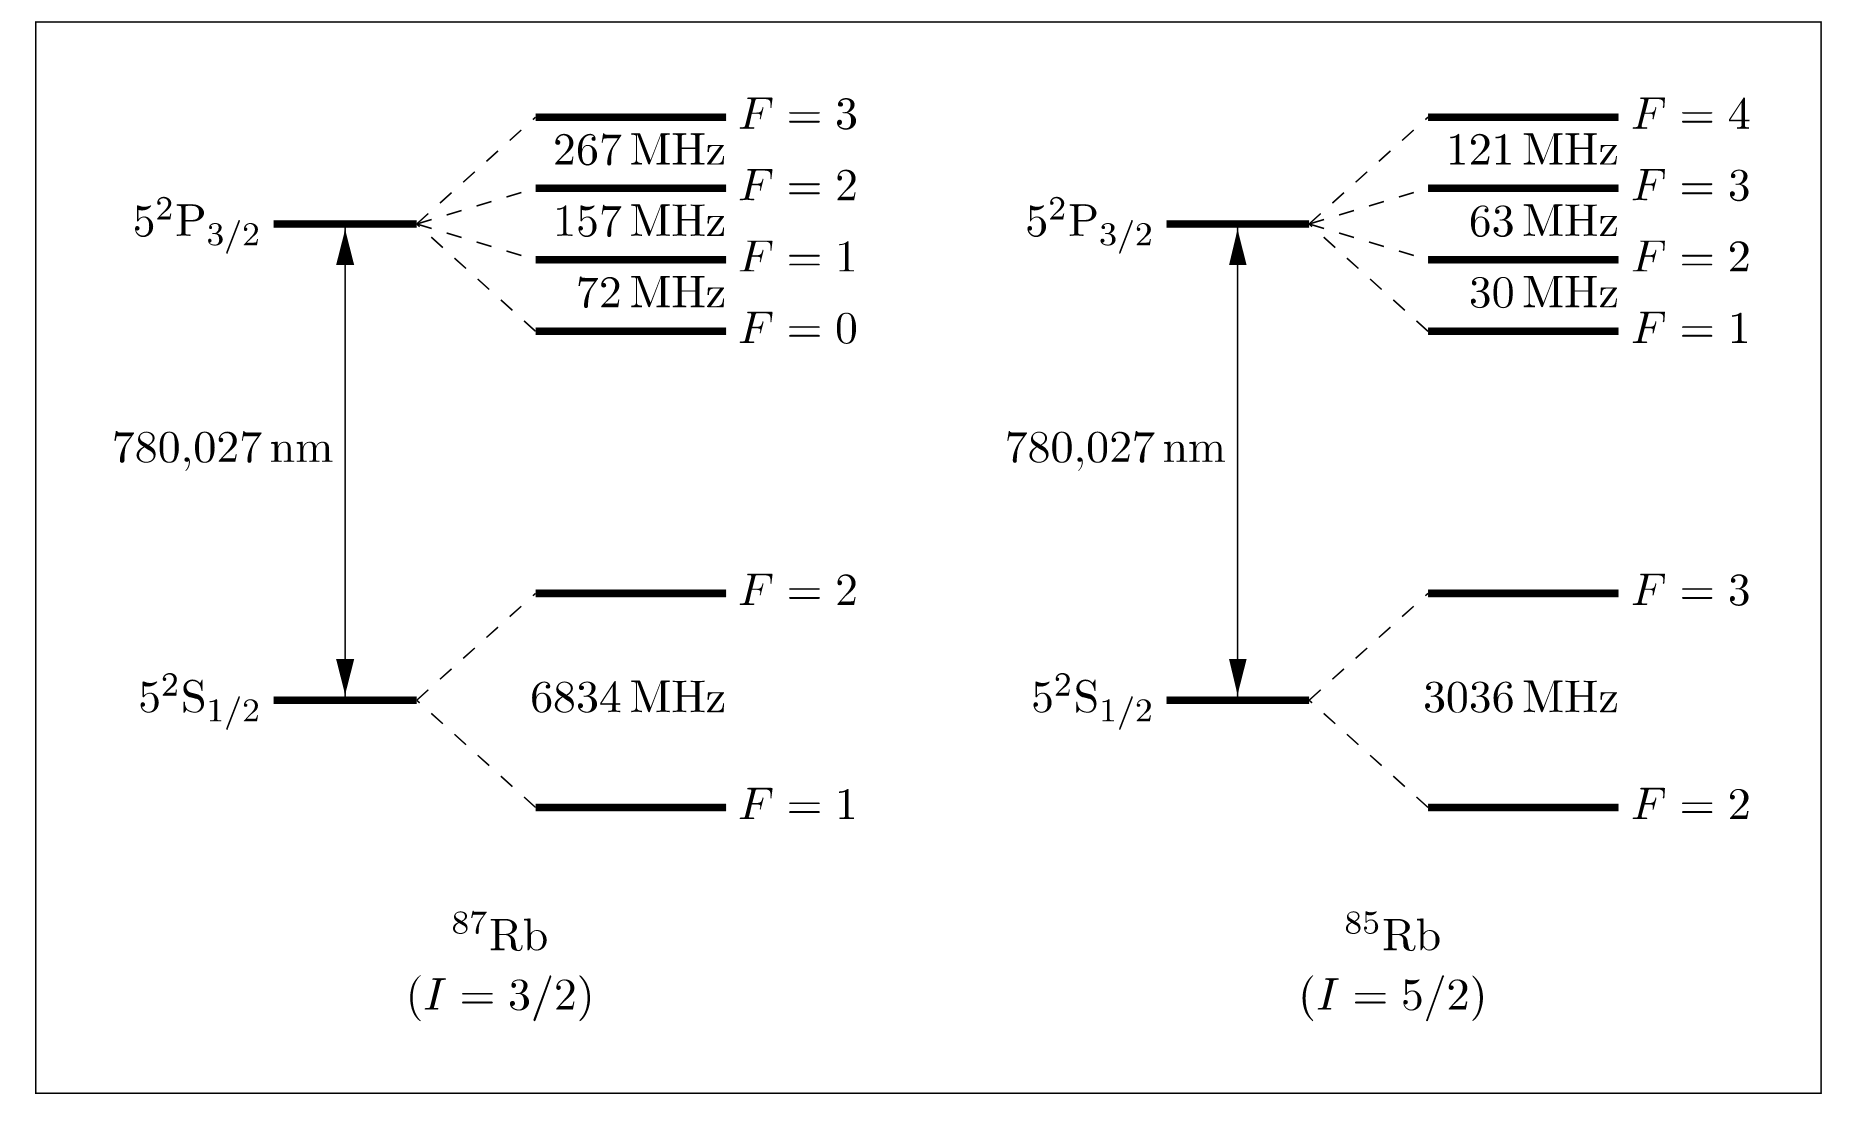
\includegraphics[width=0.9\textwidth]{level-scheme.png}
    \caption{Level scheme of Rubidium D2 transitions}
    \label{fig:level-scheme}
\end{figure}

\section{Crossover Resonances}
One challenge in SAS is the presence of crossover resonances  i.e. spectral features that do not correspond to real atomic transitions. These arise because atoms are multi-level systems, not the simple two-level systems that we have assumed.

Crossover resonances occur when both pump and probe beams interact with the same velocity class of atoms, but at different transition frequencies. These atoms absorb from both beams, leading to a dip in the spectrum at a frequency halfway between the two real transitions. The most common types are $V$, $\Lambda$, and $X$-type crossovers.

Let us consider a $V$-type crossover, involving a single ground state and two excited states with resonant frequencies $\nu_1$ and $\nu_2$. Atoms with a specific velocity class (say, 300 m/s) might see the probe at $\nu_1$ and the pump at $\nu_2$, or vice versa. Since the pump is more intense, absorption occurs preferentially from it, reducing the probe absorption and resulting in increased transmission.

This leads to a peak (typically stronger than the individual transitions) centered at $(\nu_1 + \nu_2)/2$. The key requirement is that there exist velocity classes where both beams are simultaneously resonant, which is more likely at elevated temperatures. Therefore, heating the vapor cell enhances crossover peaks.

\section{More on the Experimental Setup}

\subsection{Toptica DL100}
The laser used for this experiment was the Toptica DL100 external cavity diode laser, a tunable class 3B laser operating between 650–910 nm. Toptica provides a grating with 1800 lines/mm for this range.

A common issue encountered during tuning is \textit{mode hopping}. If the cavity length or current is not adjusted in sync with the grating angle, the laser may abruptly jump from one longitudinal mode to another. This was mitigated by adjusting the laser current and temperature. The DL100 has a coherence length of approximately 300 meters.

\subsection{Waveplates}
One of the key optical components used is a half-wave plate (HWP), often followed by a polarizing beam splitter (PBS). The HWP rotates the polarization direction of incoming linearly polarized light. When placed before a PBS, this allows precise control over the intensity and polarization of the output beams. 

\newpage

In our setup, a HWP was introduced after the optical isolator to prevent back reflections into the laser cavity. The PBS then split the beam: \textit{p}-polarized light passed through, while \textit{s}-polarized light was reflected.

An additional waveplate (HWP or QWP) was placed between mirrors M1 and M2. Rotating this waveplate changes the pump beam's polarization. This significantly affects the amplitude of spectral peaks, a phenomenon explored in Polarization Spectroscopy.

\section{Data Analysis}

\begin{figure}[htbp]
    \centering
    \includegraphics[width=1.0\textwidth]{10.png}
    \caption{SAS spectrum at 10 mW}
    \label{fig:10 mW Spectrum}
\end{figure}

\begin{figure}[!htbp]
    \centering
    \includegraphics[width=0.85\textwidth]{20.png}
    \caption{SAS spectrum at 20 mW}
    \label{fig:20_mW_Spectrum}
\end{figure}

\vspace{1em}

\begin{figure}[!htbp]
    \centering
    \includegraphics[width=0.85\textwidth]{30.png}
    \caption{SAS spectrum at 30 mW}
    \label{fig:30_mW_Spectrum}
\end{figure}

\clearpage  % forces page break here

\begin{figure}[!htbp]
    \centering
    \includegraphics[width=0.85\textwidth]{40.png}
    \caption{SAS spectrum at 40 mW}
    \label{fig:40 mW Spectrum}
\end{figure}

\vspace{1em}

\begin{figure}[!htbp]
    \centering
    \includegraphics[width=0.85\textwidth]{50.png}
    \caption{SAS spectrum at 50 mW}
    \label{fig:50 mW Spectrum}
\end{figure}

\clearpage  % another page break

\begin{figure}[!htbp]
    \centering
    \includegraphics[width=0.85\textwidth]{60.png}
    \caption{SAS spectrum at 60 mW}
    \label{fig:60 mW Spectrum}
\end{figure}

\subsection{Data Analysis}
The graphs above show experimental data collected at QuMix. The signal was obtained using a Rohde and Schwarz RTB2000 oscilloscope, displaying voltage vs. time.

\begin{itemize}
    \item First, the Doppler-broadened background and the narrow SAS features were obtained separately. The Doppler profile was subtracted to isolate the Lorentzian (saturated absorption) peaks.
    \item Baseline subtraction was performed to reduce noise. The time axis was converted to frequency, and the voltage signal was normalized to obtain absorption values.
    \item A Lorentzian function was then fit to each peak to extract the FWHM. This involved initializing parameters like the baseline (y), center frequency ($x_c$), and amplitude (A).
\end{itemize}


\newpage

\section{Further Analysis}
While fitting the peaks for FWHM is computationally involved, the results can yield valuable information about the atomic system. Additional variations include changing the pump beam’s polarization and studying the effects using polarization spectroscopy.

A promising future direction involves using vector-vortex beams and observing theirz impact on the SAS spectrum. Further experimental goals include:
\begin{itemize}
    \item Estimating the total number of atoms in the vapor cell.
    \item Calculating the absorption cross-section.
    \item Measuring the Landé $g$-factors of Rubidium.
    \item Performing precision spectroscopy to support atomic clock experiments.
\end{itemize}

\end{document}
